\documentclass{article}

% packages
\usepackage{amsmath, amsthm, thmtools, amsfonts, amssymb, luacode, catchfile, tikzducks, hyperref, ifthen}
\ifcsname c@kobocompile\endcsname
	\usepackage[a5paper, total={1072pt, 1448pt}, margin=10pt, includeheadfoot]{geometry} % set page margins
\else
	\usepackage[a4paper, margin=50pt, includeheadfoot]{geometry}
\fi
\usepackage[shortlabels]{enumitem}
\usepackage[skip=3pt, indent=0pt]{parskip}

% language
\usepackage[bidi=basic, layout=tabular, provide=*]{babel}
\ifcsname c@english\endcsname
	\babelprovide[main, import]{english}
\else
	\babelprovide[main, import]{hebrew}
	\babelprovide{rl}
\fi
%\babelfont{rm}{Libertinus Serif}
\babelfont{rm}[Renderer=Harfbuzz]{Libertinus Serif}
\babelfont{sf}{Libertinus Sans}
\babelfont{tt}{Libertinus Mono}

% style
\AddToHook{cmd/section/before}{\clearpage}	% Add line break before section
\linespread{1.3}
\setcounter{secnumdepth}{0}		% Remove default number tags from sections, this won't do well with theorems
\AtBeginDocument{\setlength{\belowdisplayskip}{3pt}}
\AtBeginDocument{\setlength{\abovedisplayskip}{3pt}}
\graphicspath{ {../images/} }

% operators
\DeclareMathOperator\cis{cis}
\DeclareMathOperator\Sp{Sp}
\DeclareMathOperator\tr{tr}
\DeclareMathOperator\im{Im}
\DeclareMathOperator\re{Re}
\DeclareMathOperator\diag{diag}
\DeclareMathOperator*\lowlim{\underline{lim}}
\DeclareMathOperator*\uplim{\overline{lim}}
\DeclareMathOperator\rng{rng}
\DeclareMathOperator\Sym{Sym}
\DeclareMathOperator\Arg{Arg}
\DeclareMathOperator\Log{Log}
\DeclareMathOperator\dom{dom}
\DeclareMathOperator\supp{Supp}
\DeclareMathOperator\var{Var}
\DeclareMathOperator\cov{Cov}

% commands
%\renewcommand\qedsymbol{\textbf{מש''ל}}
%\renewcommand\qedsymbol{\fbox{\emoji{lizard}}}
\newcommand{\Aa}[0]{\mathcal{A}}
\newcommand{\Bb}[0]{\mathcal{B}}
\newcommand{\CC}[0]{\mathbb{C}}
\newcommand{\Cc}[0]{\mathcal{C}}
\newcommand{\EE}[0]{\mathbb{E}}
\newcommand{\FF}[0]{\mathbb{F}}
\newcommand{\Ff}[0]{\mathcal{F}}
\newcommand{\Ii}[0]{\mathcal{I}}
\newcommand{\Gg}[0]{\mathcal{G}}
\newcommand{\Ll}[0]{\mathcal{L}}
\newcommand{\Mm}[0]{\mathcal{M}}
\newcommand{\NN}[0]{\mathbb{N}}
\newcommand{\Nn}[0]{\mathcal{N}}
\newcommand{\PP}[0]{\mathbb{P}}
\newcommand{\Pp}[0]{\mathcal{P}}
\newcommand{\QQ}[0]{\mathbb{Q}}
\newcommand{\RR}[0]{\mathbb{R}}
\newcommand{\Rr}[0]{\mathcal{R}}
\newcommand{\Ss}[0]{\mathcal{S}}
\newcommand{\TT}[0]{\mathbb{T}}
\newcommand{\Uu}[0]{\mathcal{U}}
\newcommand{\Vv}[0]{\mathcal{V}}
\newcommand{\Ww}[0]{\mathcal{W}}
\newcommand{\ZZ}[0]{\mathbb{Z}}
\newcommand{\acts}[0]{\circlearrowright}
\newcommand{\explain}[2] {
	\begin{flalign*}
		 && \text{#2} && \text{#1}
	\end{flalign*}
}
\newcommand{\maketitleprint}[0]{ \begin{center}
	%\begin{tikzpicture}[scale=3]
	%	\duck[graduate=gray!20!black, tassel=red!70!black]
	%\end{tikzpicture}	
	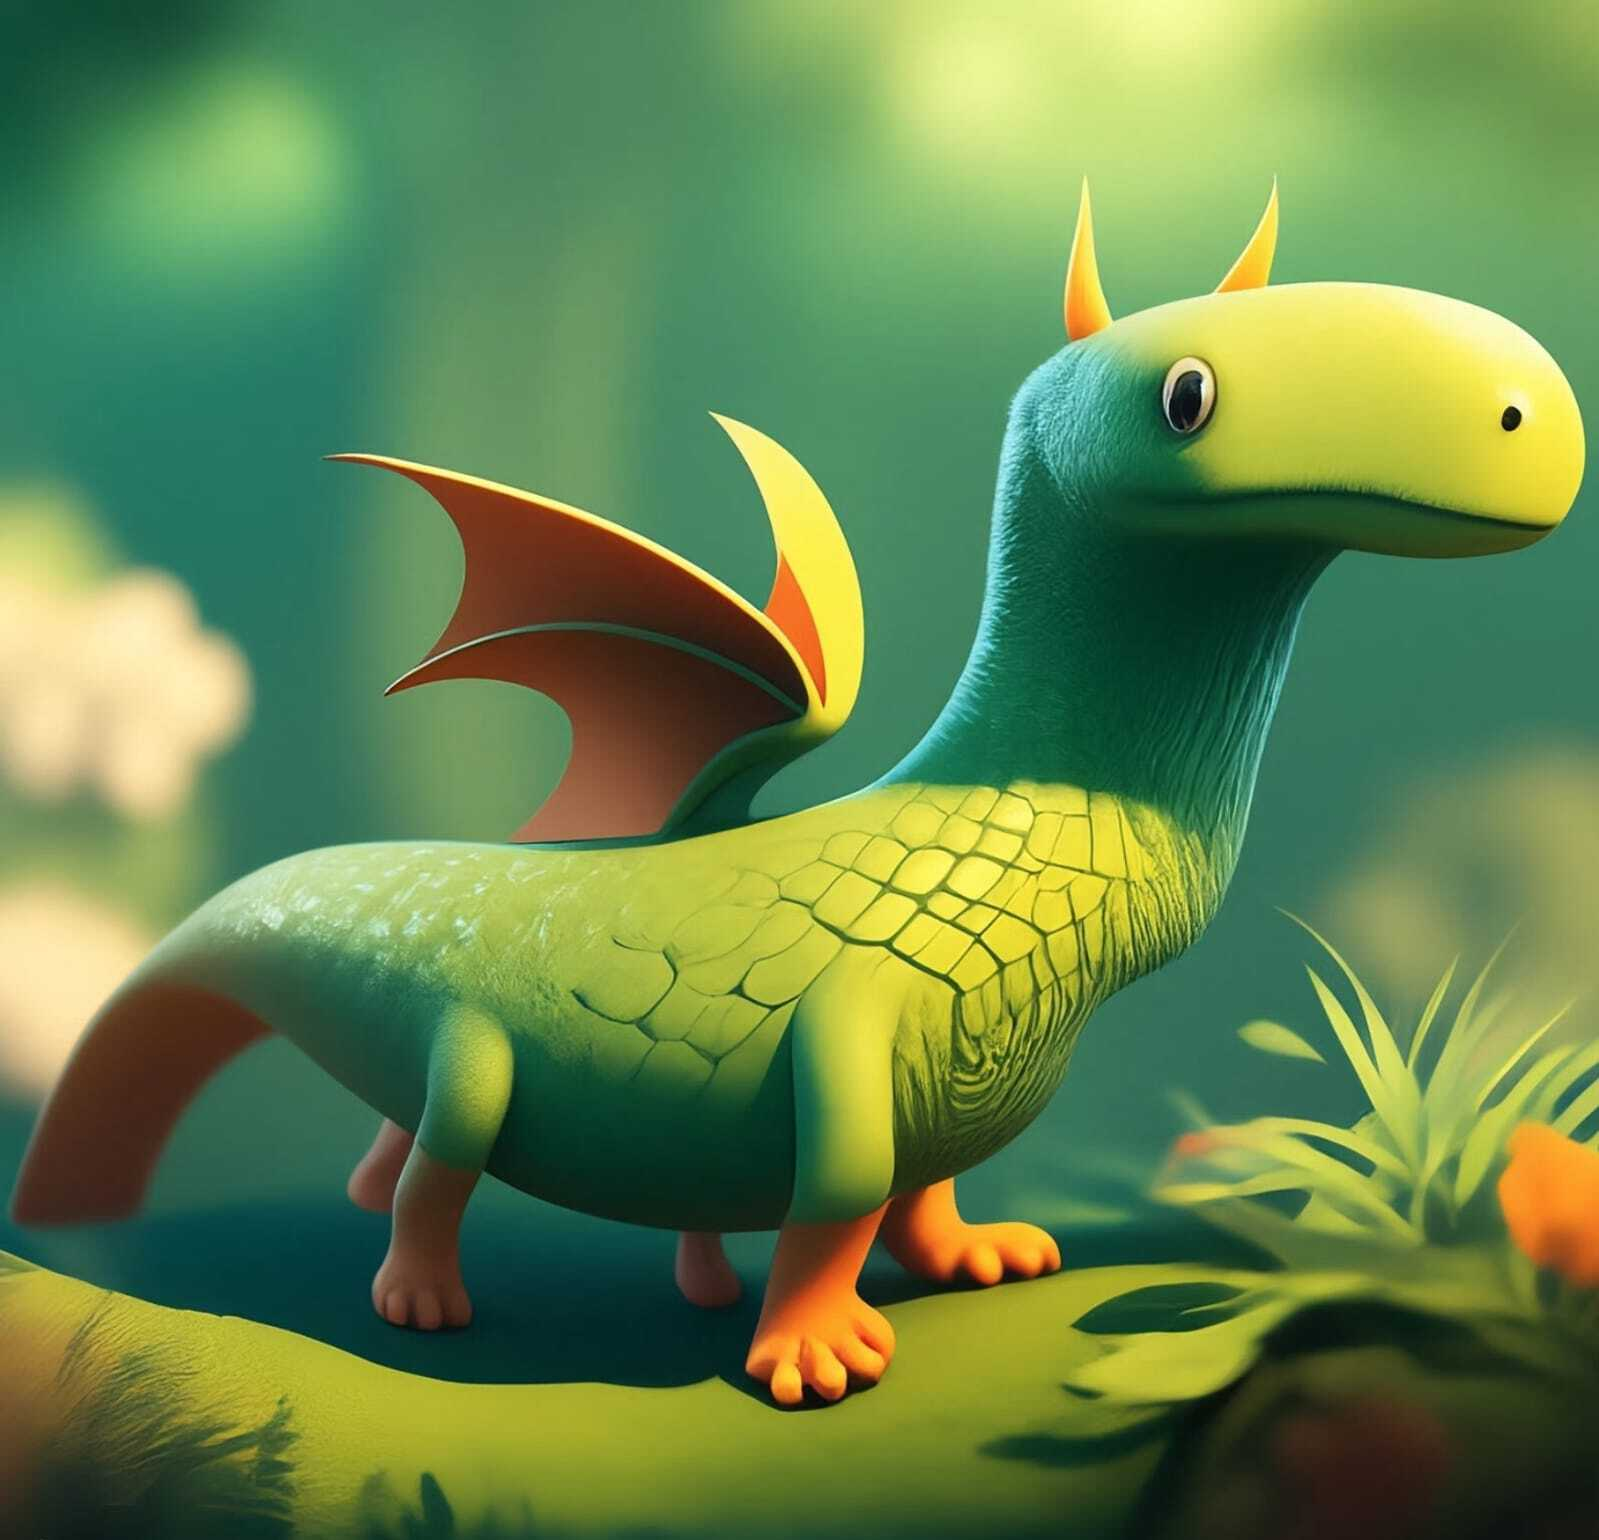
\includegraphics[width=6cm]{cover}
\end{center}
}

% theorem commands
\newtheoremstyle{c_remark}
	{}	% Space above
	{}	% Space below
	{}% Body font
	{}	% Indent amount
	{\bfseries}	% Theorem head font
	{}	% Punctuation after theorem head
	{.5em}	% Space after theorem head
	{\thmname{#1}\thmnumber{ #2}\thmnote{ \normalfont{\text{(#3)}}}}	% head content
\newtheoremstyle{c_definition}
	{3pt}	% Space above
	{3pt}	% Space below
	{}% Body font
	{}	% Indent amount
	{\bfseries}	% Theorem head font
	{}	% Punctuation after theorem head
	{.5em}	% Space after theorem head
	{\thmname{#1}\thmnumber{ #2}\thmnote{ \normalfont{\text{(#3)}}}}	% head content
\newtheoremstyle{c_plain}
	{3pt}	% Space above
	{3pt}	% Space below
	{\itshape}% Body font
	{}	% Indent amount
	{\bfseries}	% Theorem head font
	{}	% Punctuation after theorem head
	{.5em}	% Space after theorem head
	{\thmname{#1}\thmnumber{ #2}\thmnote{ \text{(#3)}}}	% head content

\ifcsname c@english\endcsname
	\theoremstyle{plain}
	\newtheorem{theorem}{Theorem}[section]
	\newtheorem{lemma}[theorem]{Lemma}
	\newtheorem{proposition}[theorem]{Proposition}
	\newtheorem*{proposition*}{Proposition}
	%\newtheorem{corollary}[theorem]{אין חלופה עברית}

	\theoremstyle{definition}
	\newtheorem{definition}[theorem]{Definition}
	\newtheorem*{definition*}{Definition}
	\newtheorem{example}{Example}[section]
	\newtheorem{exercise}{Exercise}[section]

	\theoremstyle{remark}
	\newtheorem*{remark}{Remark}
	\newtheorem*{solution}{Solution}
	\newtheorem{conclusion}[theorem]{Conclusion}
	\newtheorem{notation}[theorem]{Notation}
\else
	\theoremstyle{c_plain}
	\newtheorem{theorem}{משפט}[section]
	\newtheorem{lemma}[theorem]{למה}
	\newtheorem{proposition}[theorem]{טענה}
	\newtheorem*{proposition*}{טענה}
	%\newtheorem{corollary}[theorem]{אין חלופה עברית}

	\theoremstyle{c_definition}
	\newtheorem{definition}[theorem]{הגדרה}
	\newtheorem*{definition*}{הגדרה}
	\newtheorem{example}{דוגמה}[section]
	\newtheorem{exercise}{תרגיל}[section]

	\theoremstyle{c_remark}
	\newtheorem*{remark}{הערה}
	\newtheorem*{solution}{פתרון}
	\newtheorem{conclusion}[theorem]{מסקנה}
	\newtheorem{notation}[theorem]{סימון}
\fi

% Questions related commands
\newcounter{question}
\setcounter{question}{1}
\newcounter{sub_question}
\setcounter{sub_question}{1}

\ifcsname c@english\endcsname
	\newcommand{\question}[1][0]{
		\ifthenelse{#1 = 0}{}{\setcounter{question}{#1}}
		\section{Question \arabic{question}}
		\addtocounter{question}{1}
		\setcounter{sub_question}{1}
	}

	\newcommand{\subquestion}[1][0]{
		\ifthenelse{#1 = 0}{}{\setcounter{sub_question}{#1}}
		\subsection{Part \alph{sub_question}}
		\addtocounter{sub_question}{1}
	}
\else
	\newcommand{\question}[1][0]{
		\ifthenelse{#1 = 0}{}{\setcounter{question}{#1}}
		\section{שאלה \arabic{question}}
		\addtocounter{question}{1}
		\setcounter{sub_question}{1}
	}

	\newcommand{\subquestion}[1][0]{
		\ifthenelse{#1 = 0}{}{\setcounter{sub_question}{#1}}
		\subsection{סעיף \localecounter{letters.gershayim}{sub_question}}
		\addtocounter{sub_question}{1}
	}
\fi

% import lua and start of document
\directlua{common = require ('../common')}

\GetEnv{AUTHOR}

% headers
\author{\AUTHOR}
\date\today

\title{פתרון מטלה 07 --- תורת ההסתברות (1), 80420}

\DeclareMathOperator{\Supp}{Supp}

\begin{document}
\maketitle
\maketitleprint{}

\question{}
נוכיח או נפריך את הטענות הבאות.

\subquestion{}
נסתור את הטענה שאם יהי $X$ משתנה מקרי המוגדר על מרחב ההסתברות $(\Omega, \PP)$, ונניח ש־$X \sim U(\{1, 2, 3\})$, אז $(\Omega, \PP)$ הוא מרחב הסתברות אחידה.
\begin{solution}
	נניח שמרחב ההסתברות הוא של הטלת קובייה לא אחידה כך שלקבלת המספרים הזוגיים הסתברות של חצי מקבלת המספרים האי־זוגיים, כאשר ההסתברות אחידה בין מספרים עם אותה הזוגיות. \\*
	נגדיר גם $X(1) = X(2) = 1, X(3) = X(4) = 2, X(5) = X(6) = 3$, אז $X \sim U(\{1, 2, 3\})$ בעוד מרחב ההסתברות לא אחיד.
\end{solution}

\subquestion{}
יהיו $X, Y$ משתנים מקריים בלתי־תלויים ובעלי תומך סופי.
נסתור את הטענה שאם $\EE(|X - Y|) = 0$ אז $\PP(X = Y) = 1$.
\begin{solution}
	נגדיר $\Omega = \{-1, 1\}$ וכן $X(\omega) = \omega, Y(\omega) = -\omega$, לכן $\EE(|X - Y|) = 0$, אבל $\PP(X = Y) = 0 \ne 1$.
\end{solution}

\subquestion{}
נסתור את הטענה שאם נניח ש־$X$ משתנה מקרי בעל תוחלת, אז גם $X^2$ בעל תוחלת.
\begin{solution}
	נניח ש־$\Supp X = \NN$ וכן $\PP(X = n) = \frac{c}{n^3}$, ראינו כי אכן קיים משתנה מקרי כזה עם התפלגות כזו בהרצאות קודמות, ואנו יודעים כי
	\[
		\EE(X) = \sum_{n = 1}^{\infty} n \cdot \frac{c}{n^3}
	\]
	הוא טור מתכנס בהחלט, לעומת זאת
	\[
		\EE(X) = \sum_{n = 1}^{\infty} n^2 \cdot \frac{c}{n^3}
	\]
	הוא טור הרמוני ומתבדר.
\end{solution}

\subquestion{}
נניח ש־$X$ משתנה מקרי כך ש־$X^2$ הוא בעל תוחלת, נוכיח שגם $X$ בעל תוחלת.
\begin{solution}
	מתקיים
	\begin{align*}
		\EE(X^2)
		& = \sum_{s \in \RR_{\ge 0}} s \PP(X^2 = s) \\
		& = \sum_{s \in \RR_{\ge 0}} \sqrt{s} \cdot \sqrt{s} \PP(X \in \{\sqrt{s}, -\sqrt{s}\}) \\
		& = \sum_{s' \in \RR_{\ge 0}} s' \cdot s' \PP(X \in \{s', -s'\}) \\
		& = \sum_{s' \in \RR_{\ge 0}} s' \cdot s' (\PP(X = s') + \PP(X = -s')) \\
		& = \sum_{s' \in \RR_{\ge 0}} s' \cdot s' \PP(X = s') + \sum_{s' \in \RR_{\ge 0}} s' \cdot s' \PP(X = s') \\
		& = \sum_{s' \in \RR_{\ge 0}} |s'| \cdot |s' \PP(X = s')| + \sum_{s' \in \RR_{< 0}} |s'| \cdot |s' \PP(X = s')| \\
		& = \sum_{s' \in \RR} |s'| \cdot |s' \PP(X = s')| \\
		& = \sum_{s \in \supp X} |s| \cdot |s \PP(X = s)|
	\end{align*}
	הוא טור מתכנס בהחלט, ולכן ממבחן התכנסות גם
	\[
		\sum_{s \in S} |s \PP(X = s)|
	\]
	טור מתכנס, אבל זוהי התכנסות בהחלט של $\EE(X)$ עצמו, קרי יש תוחלת ל־$X$.
\end{solution}

\subquestion{}
יהיו $X, Y$ משתנים מקריים כך ש־$\EE(X) = \EE(Y)$ וכן $\EE(X^2) = \EE(Y^2)$.
נסתור את הטענה שאז $\PP(X = Y) = 1$.
\begin{solution}
	נניח שוב ש־$X, Y$ קבועים כך ש־$X = 1, Y = 2$ כמעט תמיד. \\*
	אז כמובן התוחלת שלהם ושל הריבוע שלהם שווה, אבל $\PP(X = Y) = 0$.
\end{solution}

\subquestion{}
נסתור את הטענה כי קיים משתנה מקרי בדיד $X$ אי־שלילי בעל תוחלת סופית כך שמתקיים
\[
	\exists N \in \NN, \forall n \ge N, \PP(X \ge n) = \frac{\EE(X)}{n}
\]
\begin{proof}
	נניח בשלילה שאכן קיים משתנה מקרי $X$ כזה.
	נובע אם כך עבור ההסתברות שלו עבור $n > N + 1$,
	\[
		\PP(X = n)
		= \PP(X \ge n) - \PP(X \ge n - 1)
		= \frac{\EE(X)}{n} - \frac{\EE(X)}{n - 1}
		= \EE(X) \frac{-1}{n(n - 1)}
	\]
	ולכן מהגדרת התוחלת
	\[
		\EE(X)
		= \sum_{n \in \NN} n \PP(n)
		= \sum_{n = 1}^{N} n \PP(X = n) + \sum_{n \in \NN} \EE(X) \frac{-1}{n - 1}
	\]
	נסמן $C = \sum_{n = 1}^{N} n \PP(X = n)$ ונבחין כי $C \ge 0$ וסופי בפרט, אבל
	\[
		C = \EE(X) (1 + \sum_{n = N + 1}^{\infty} \frac{1}{n - 1})
	\]
	וזו כמובן סתירה מהתבדרות הטור ההרמוני, לכן $\EE(X) = 0$. נעיר שמהנתון התומך הוא לא סופי, אחרת הטענה לא מתקיימת. \\*
	נניח ש־$\EE(X) = 0$, לכן מהנתון התפלגות $X$ קבועה, ובהתאם לאינסופיות התומך היא 0 בלבד, אבל זאת סתירה להגדרת התפלגות, ולכן קיבלנו סתירה.
\end{proof}

\question{}
במשחק מטילים מטבע הוגן עד שמקבלים תוצאה של עץ. אם העץ המתקבל בהטלה ה־$i$ אז מוענקים למטיל $a^i$ נקודות.

\subquestion{}
יהי $X$ המשתנה המקרי המתאר את כמות הנקודות שהוענקה, נחשב את התפלגות $X$
\begin{solution}
	נבחין כי מההגדרה המשתנה $Y$ המתאר את השאלה באיזה סיבוב המשחק הסתיים הוא $Geo(\frac{1}{2})$. \\*
	בהתאם $X = a^Y$, שכן כמות הנקודות המתקבלת היא מספר הסיבוב האחרון כחזקת $a$. \\*
	נעבור אם כן לחישוב ההתפלגות של $X$:
	\[
		\PP(X = n)
		= \PP(a^Y = n)
		= \PP(Y = \log_a n)
		= {(1 - \frac{1}{2})}^{\log_a(n) - 1} \cdot \frac{1}{2}
		= \frac{1}{2^{\log_a n}}
	\]
	נבחין כי התומך הוא $\supp X = \{ a^n \mid n \in \NN \}$.
\end{solution}

\subquestion{}
נחשב את $\EE(X)$ לכל $a$.
\begin{solution}
	\[
		\EE(X)
		= \sum_{s \in \Supp X} s \cdot \PP(X = s)
		= \sum_{n = 1}^\infty a^n \cdot \frac{1}{2^{\log_a a^n}}
		= \sum_{n = 1}^\infty {\left(\frac{a}{2}\right)}^n
		= \frac{\frac{a}{2}}{1 - \frac{a}{2}}
		= \frac{a}{2 - a}
	\]
\end{solution}

\subquestion{}
נחשב את ההסתברות להרוויח יותר מעשר נקודות עבור $a = 2$.
\begin{solution}
	נבחין כי $X = 2^4$ הוא המקרה הראשון שבו מתקבלות מעל 10 נקודות, לכן אנו מחפשים את
	\[
		\PP(X \ge 10) = \PP(Y \ge \log_2 10) = 1 - \PP(1 \le Y \le 3) = 1 - \PP(Y = 1) - \PP(Y = 2) - \PP(Y = 3) = 1 - \frac{1}{2^1} - \frac{1}{2^2} - \frac{1}{2^3} = \frac{1}{8}
	\]
\end{solution}

\question{}
\subquestion{}
ישנן שלוש צנצנות עוגיות, בראשונה 15 עוגיות, בשנייה 18 ובשלישית 9.

\subsubsection{i}
בוחרים עוגייה באופן אקראי ואחיד, נחשב את התוחלת של מספר העוגיות בצנצנת שלה.
\begin{solution}
	אם נמספר את העוגיות נקבל 42 עוגיות, ונגדיר את המשתנה המקרי $X$ כמחזיר לכל מספר עוגייה את מספר העוגיות בצנצנת שלה, כך לדוגמה $X(1) = 15$ וכן הלאה. \\*
	בהתאם נקבל
	\[
		\EE(X)
		= \sum_{i = \{15, 18, 9\}} i \PP(X = i)
		= 15 \cdot \frac{15}{42} + 18 \cdot \frac{18}{42} + 9 \cdot \frac{9}{42}
	\]
\end{solution}

\subsubsection{ii}
בוחרים צנצנת באקראי ובאופן אחיד, נחשב את התוחלת של מספר העוגיות בצנצנת שבחרנו.
\begin{solution}
	הפעם נגדיר $Y$ מחזיר את מספר העוגיות עבור מספר צנצנת, כלומר $Y(1) = 15$ וכדומה, לכן
	\[
		\EE(Y) = \frac{1}{3} \cdot 15 + \frac{1}{3} \cdot 18 + \frac{1}{3} \cdot 9
	\]
\end{solution}

\subquestion{}
מטילים שתי קוביות הוגנות.
נמצא את תוחלת סכום התוצאות של הקוביות בהינתן שהקוביות נפלו על פאות שונות.
\begin{solution}
	נגדיר $X, Y$ תוצאת הטלת שתי הקוביות, ונגדיר גם $Z = X + Y \mid X \ne Y$. \\*
	הסכום יכול לצאת במקרה זה בין 3 ל־11, דהינו $\supp Z = \{3, \dots, 11\}$, ולכן
	\[
		\EE(Z)
		= \sum_{i = 3}^{11} i \PP(Z = i)
		= 3 \cdot \frac{2}{36} + \cdots + 11 \cdot \frac{2}{36}
	\]
\end{solution}

\subquestion{}
מטילים קובייה הוגנת שוב ושוב עד שיוצאת התוצאה 6. \\*
יהי $X$ המשתנה המקרי המייצג את מספר הפעמים שהתקבלה התוצאה 2. \\*
נחשב את התוחלת של $X$ בהינתן שכל ההטלות היו זוגיות.
\begin{solution}
	נגדיר $Y$ שיצא 6 בתוצאה ה־$i$, לכן $Y \sim Geo(\frac{1}{6})$. \\*
	בנוסף נגדיר $X$ המשתנה המקרי המייצג את מספר ה־2 שהתקבלו, נבחין כי $Z \mid A, Y = n \sim Bin(n - 1, \frac{1}{2})$, ישירות מכלל הסידורים האפשריים של הטלות. \\*
	מנוסחת התוחלת השלמה
	\[
		\EE(Z \mid A)
		= \sum_{n = 1}^{\infty} \EE(Z \mid A, Y = n) \PP(Y = n \mid A)
	\]
	נעבור אם כך לחישוב ערכים אלה.
	\[
		\PP(Y = n \mid A)
		= \frac{\PP(Y = n, A)}{\PP(A)}
		= \frac{\PP(Y = n, A)}{\PP(A)}
	\]
	וכן
	\[
		\PP(Y = n, A)
		= {(\frac{2}{6})}^{n - 1} \frac{1}{6}
	\]
	ולכן גם
	\[
		\PP(A)
		= \sum_{n = 1}^{\infty} \PP(Y = n, A)
		= \sum_{n = 1}^{\infty} {(\frac{1}{3})}^{n - 1} \frac{1}{6}
		= \frac{1}{6} \cdot \frac{1}{1 - \frac{1}{3}}
		= \frac{1}{4}
	\]
	ומצאנו ש־$\PP(Y = n \mid A) = \frac{\frac{1}{3^{n - 1}} \frac{1}{6}}{\frac{1}{4}} = \frac{1}{3^{n - 1}} \frac{2}{3}$, דהינו $Y \mid A \sim Geo(\frac{2}{3})$. \\*
	אנו גם יודעים ש־$Z \mid A, Y = n \sim Bin(n - 1, \frac{1}{2})$ ולכן $\EE(Z \mid A, Y = n) = (n - 1) \frac{1}{2}$ ובהתאם
	\[
		\EE(Z \mid A)
		= \sum_{n = 1}^{\infty} \frac{n - 1}{2} \PP(Y = n \mid A)
		= \frac{1}{2} \sum_{n = 1}^{\infty} (n - 1) \PP(Y = n \mid A)
		= \frac{1}{2} (\EE(Y \mid A) - \sum_{n = 1}^{\infty} \PP(Y = n \mid A))
		= \frac{1}{2} (\frac{3}{2} - 1)
		= \frac{1}{4}
	\]
\end{solution}

\subquestion{}
עשרה שופטים בתחרות מעניקים לקבוצת אנשים ציונים מקריים המתפלגים אחיד ב־$[10]$. \\*
נחשב את תוחלת הציון המינימלי והציון המקסימלי שקיבלה הקבוצה.
\begin{solution}
	נגדיר $\forall i \in [10], X_i \sim U([10])$ הציון שנתן השופט ה־$i$. בנוסף נגדיר $X = \min\{ X_1, \dots, X_{10} \}$ הציון המינימלי. \\*
	נבחין כי $\{ \omega \in \Omega \mid X(\omega) \ge n \} = \{ \omega \in \Omega \mid X_i(\omega_i) \ge n \}$ ולכן
	\[
		\PP(X \ge n)
		= {\left(\frac{10 - (n - 1)}{10}\right)}^{10}
	\]
	ולכן מנוסחת הזנב
	\[
		\EE(X)
		= \sum_{n = 1}^{10} \PP(X \ge n)
		= \sum_{n = 1}^{10} {\left(\frac{10 - (n - 1)}{10}\right)}^{10}
		\approx 1.49
	\]
	באופו דומה נגדיר $Y = \max\{ X_1, \dots, X_{10} \}$, ולכן
	\[
		\PP(Y \ge n)
		= 1 - \PP(Y < n)
		= 1 - {\left(\frac{n - 1}{10}\right)}^{10}
	\]
	וכן
	\[
		\EE(Y)
		= \sum_{n = 1}^{10} \PP(Y \ge n)
		= \sum_{n = 1}^{10} 1 - {\left(\frac{n - 1}{10}\right)}^{10}
		\approx 9.50
	\]
\end{solution}

\question{}
יהי משתנה מקרי בעל תוחלת $X$ הנתמך על $\NN$. \\*
נוכיח כי $X \sim Geo(p)$ עבור $p \in (0, 1)$ כלשהו אם ורק אם לכל $s \in \NN \cup \{0\}$ מתקיים
\[
	\EE(X \mid X > s) = \EE(X) + s
\]
\begin{proof}
	נניח ש־$X \sim Geo(p)$ ולכן תכונת חוסר הזיכרון מתקיימת, כלומר נובע $X \overset{d}{=} X - s \mid X > s$ לכל $s$ בתחום. \\*
	נחשב
	\begin{align*}
		\EE(X \mid X > s)
		& = \sum_{n = 1}^{\infty} n \PP(X - s = n - s \mid X > s) \\
		& = \sum_{n = s + 1}^{\infty} n \PP(X - s = n - s \mid X > s) \\
		& = \sum_{n = s + 1}^{\infty} n \PP(X = n - s) \\
		& = \sum_{n = s + 1}^\infty n \cdot {(1 - p)}^{n - s - 1} p
	\end{align*}
	ומצד שני
	\[
		\EE(X) + s
		= \frac{s p}{1 - (1 - p)} + \sum_{n = 1}^{\infty} n {(1 - p)}^{n - 1} p
		= \sum_{n = 1}^{\infty} {(1 - p)}^{n - 1} s p + \sum_{n = 1}^{\infty} n {(1 - p)}^{n - 1} p
		= \sum_{n = 1}^{\infty} (n + s) {(1 - p)}^{n - 1} p
	\]
	ומצאנו כי הביטויים שווים.

	נניח את הכיוון השני של הטענה, אז הטענה נכונה גם עבור $s = 1$, כלומר
	\[
		\EE(X \mid X > 1) = \EE(X) + 1
	\]
	לכן
	\[
		\EE(X - 1 \mid X > 1)
		= \sum_{n = 1}^{\infty} n \PP(X - 1 = n \mid X > 1)
		= \sum_{n = 2}^{\infty} (n - 1) \PP(X = n \mid X > 1)
		= \EE(X \mid X > 1) - 1
		= \EE(X)
	\]
	ואז $\EE(X - 1 \mid X > 1) - \EE(X) = 0$, ומההתכנסות בהחלט ואינדוקציה על $n$ נקבל משקילות תכונת חוסר הזיכרון את המבוקש.
\end{proof}

\question{}
נמצא דוגמה לשני משתנים מקריים בעלי תוחלת תלויים כך ש־$\EE(X \cdot Y) = \EE(X) \cdot \EE(Y)$.
\begin{solution}
	נגדיר $X = Y \sim Ber(1)$ ולכן
	\[
		\EE(XY)
		= \EE(X^2)
		= \sum_{n \in \{0, 1\}} n^2 \PP(X = n)
		= 0 \cdot (1 - 1) + 1 \cdot 1
		= 1
	\]
	ומצד שני
	\[
		\EE(X) \cdot \EE(Y)
		= {(\EE(X))}^2
		= 1^2
		= 1
	\]
	ומצאנו כי הטענה מתקיימת.
\end{solution}

\end{document}
